% Created 2026-04-23 Thu 12:08
% Intended LaTeX compiler: lualatex
\DocumentMetadata{lang = en-US,pdfversion = 2.0,pdfstandard = ua-2,tagging = on,tagging-setup = {math/setup=mathml-SE},}
\documentclass[11pt]{article}
\usepackage{amsmath}
\usepackage{fontspec}
\usepackage{graphicx}
\usepackage{longtable}
\usepackage{wrapfig}
\usepackage{rotating}
\usepackage[normalem]{ulem}
\usepackage{capt-of}
\usepackage{hyperref}
\usepackage[margin=1in]{geometry}
\usepackage{fontspec}
\usepackage{verbatim, multicol, tabularx,}
\usepackage{amsmath, amsthm, amssymb, stmaryrd, latexsym, bm, listings, qtree}
\usepackage{framed}
\usepackage{xcolor,colortbl}
\usepackage{media9}
\usepackage[export]{adjustbox}
\usepackage{algorithm}
\usepackage[noend]{algpseudocode}
\usepackage{tikz,pgfplots}
\usetikzlibrary{shapes.geometric}
\let\oldquote=\quote
\let\endoldquote=\endquote
\colorlet{shadecolor}{cyan!15}
\renewenvironment{quote}{\begin{shaded*}\begin{oldquote}}{\end{oldquote}\end{shaded*}}
% From https://tex.stackexchange.com/questions/7032/good-way-to-make-textcircled-numbers
\newcommand*\circled[1]{\tikz[baseline=(char.base)]{\node[shape=circle,draw,inner sep=2pt] (char) {#1};}}
\DeclareMathOperator*{\argmin}{arg\!min}
\DeclareMathOperator*{\argmax}{arg\!max}
\lstset{frame=tb, aboveskip=1mm, belowskip=0mm, showstringspaces=false, columns=flexible, basicstyle={\scriptsize\ttfamily}, numbers=left, frame=single, breaklines=true, breakatwhitespace=true}
\hypersetup{colorlinks=true,urlcolor=blue}
\usepackage{tagpdf}
\tagpdfsetup{activate-all}
\tagpdfsetup{math/alt/use}
\usepackage{polyglossia}
\setdefaultlanguage[variant=en-US]{english}
\author{Christopher Simpkins}
\date{Kennesaw State University}
\title{Artificial Intelligence\\\medskip
\large Machine Learning}
\hypersetup{
 pdfauthor={Christopher Simpkins},
 pdftitle={Artificial Intelligence},
 pdfkeywords={},
 pdfsubject={Artificial Intelligence Machine Learning},
 pdfcreator={Emacs 30.2 (Org mode 9.7.11)}, 
 pdflang={English}}
\begin{document}

\maketitle
\section{What is machine learning?}
\label{sec:orgbd3903f}

Definition by Tom Mitchell (1998):

Machine Learning is the study of algorithms that

\begin{itemize}
\item improve their performance \texttt{P}
\item at some task \texttt{T}
\item with experience \texttt{E}.
\end{itemize}

A well-defined learning task is given by ``.
\section{Examples of Machine Learning Tasks [\textsuperscript{mooney}]}
\label{sec:orgfa10237}

Improve on task \texttt{T}, with performance \texttt{P}, given experience \texttt{E}

\texttt{T}: Playing checkers

\begin{itemize}
\item \texttt{P}: Percentage of games won against an arbitrary opponent
\item \texttt{E}: Playing practice games against itself
\end{itemize}

\texttt{T}: Recognizing hand-written words

\begin{itemize}
\item \texttt{P}: Percentage of words correctly classified
\item \texttt{E}: Database of human-labeled images of handwritten words
\end{itemize}

\texttt{T}: Driving on four-lane highways using vision sensors

\begin{itemize}
\item \texttt{P}: Average distance traveled before a human-judged error
\item \texttt{E}: A sequence of images and steering commands recorded while observing a human driver.
\end{itemize}

\texttt{T}: Categorize email messages as spam or legitimate.

\begin{itemize}
\item \texttt{P}: Percentage of email messages correctly classified.
\item \texttt{E}: Database of emails, some with human-given labels
\end{itemize}

{[}\textsuperscript{mooney}]: Slide credit: Ray Mooney
\section{Elements of Machine Learning Problems}
\label{sec:orgf90c1dd}

Every machine learning problem includes

\begin{itemize}
\item data from which to learn,
\item a model that takes input data and produces an "answer",
\item an error function that quantifies the badness of our model, and
\item an algorithm that adjusts the model’s parameters to minimize a loss function.
\begin{itemize}
\item A loss function is a surrogate of the error function used by the algorithm.  It may be the error function itself, but is often some closely related function with desirable mathematical properties.
\end{itemize}
\end{itemize}

Our model, or hypothesis, comes from a model/hypothesis class.  Once the parameters are learned, we have an instance of the hypothesis class tuned to our particular machine learning problem.
\section{Kinds of Machine Learning Tasks}
\label{sec:orgbb6a3e6}

\begin{itemize}
\item Classification: identify the correct label for an instance
\begin{itemize}
\item Does this image contain a dog/peron on no-fly list/lung tumor?
\item Which radio emitted the signal we received?
\item Will this customer respond to this advertisement?
\end{itemize}

\item Clustering: identify the groups into which instances fall
\begin{itemize}
\item What are the discernible groups of \ldots{} customers, cars, colors in an images
\item Is this operating state similar to known operating states, or is it an anomaly?
\end{itemize}

\item Agent behavior
\begin{itemize}
\item Given the state, which action should the agent take to maximize its goal attainment?
\end{itemize}

\item Generation
\begin{itemize}
\item Given a prompt, generate an image/video/poem/love letter.
\end{itemize}
\end{itemize}
\section{Kinds of Machine Learning Algorithms}
\label{sec:orgeea52d4}

\begin{itemize}
\item Supervised
\begin{itemize}
\item Learn from a training set of labeled data -- the supervisor
\item Generalize to unseen instances
\end{itemize}

\item Unsupervised
\begin{itemize}
\item Learn from a set of unlabeled data
\item Place an unseen instance into appropriate group
\item Infer rules describing the groups
\end{itemize}

\item Reinforcement learning
\begin{itemize}
\item Learn from a history of trial-and-error exploration
\item Output is a \textbf{policy} -- a mapping from states to actions (or probability distributions over actions)
\end{itemize}
\end{itemize}

Classification using supervised learning methods makes up the lion's share of machine learning.
\section{Supervised Learning Problem Setup}
\label{sec:org447be2f}

Every machine learning problem contains the following elements:

\begin{itemize}
\item An input \(\vec{x}\)
\item An unkown target function \(f: \mathcal{X} \rightarrow \mathcal{Y}\)
\item A data set \(\mathcal{D}\)
\item A learning model, which consists of
\begin{itemize}
\item a hypothesis class \(\mathcal{H}\), and
\item a learning algorithm.
\end{itemize}
\end{itemize}

A learning algorithm uses elements of \(\mathcal{D}\) to estimate parameters of of a particular \(h(\vec{x})\) from \(\mathcal{H}\) which maps every \(\vec{x}\) to an element of \(\mathcal{Y}\).
\section{Classification Example}
\label{sec:org0a45966}

Classification is a supervised learning task in which the target function maps feature vectors in \(\mathbb{R}^{d}\) to one of a defined set of classes.

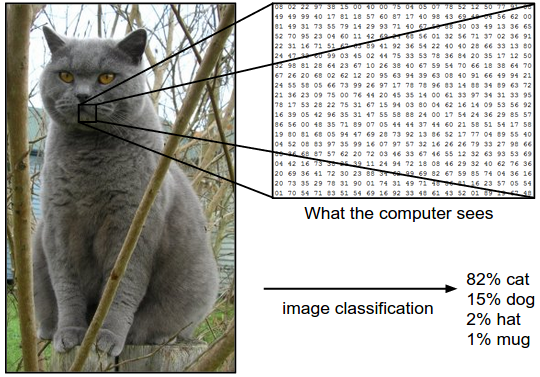
\includegraphics[alt={../../deep learning/slides/cat classify},height=2.0in]{../../deep-learning/slides/cat-classify.png}

\begin{itemize}
\item In linear classification we assume that there are lines that separates classes acceptably well.
\begin{itemize}
\item Binary: two classes
\item Multiclass: more than two classes
\end{itemize}
\end{itemize}

{[}\textsuperscript{cs231n}]: \url{https://cs231n.github.io/classification/}
\section{Regression Example}
\label{sec:org3f8ad9d}

Regression is a kind of supervised learning in which the target function maps feature vectors in \(\mathbb{R}^{d}\) to arbitrary real values.

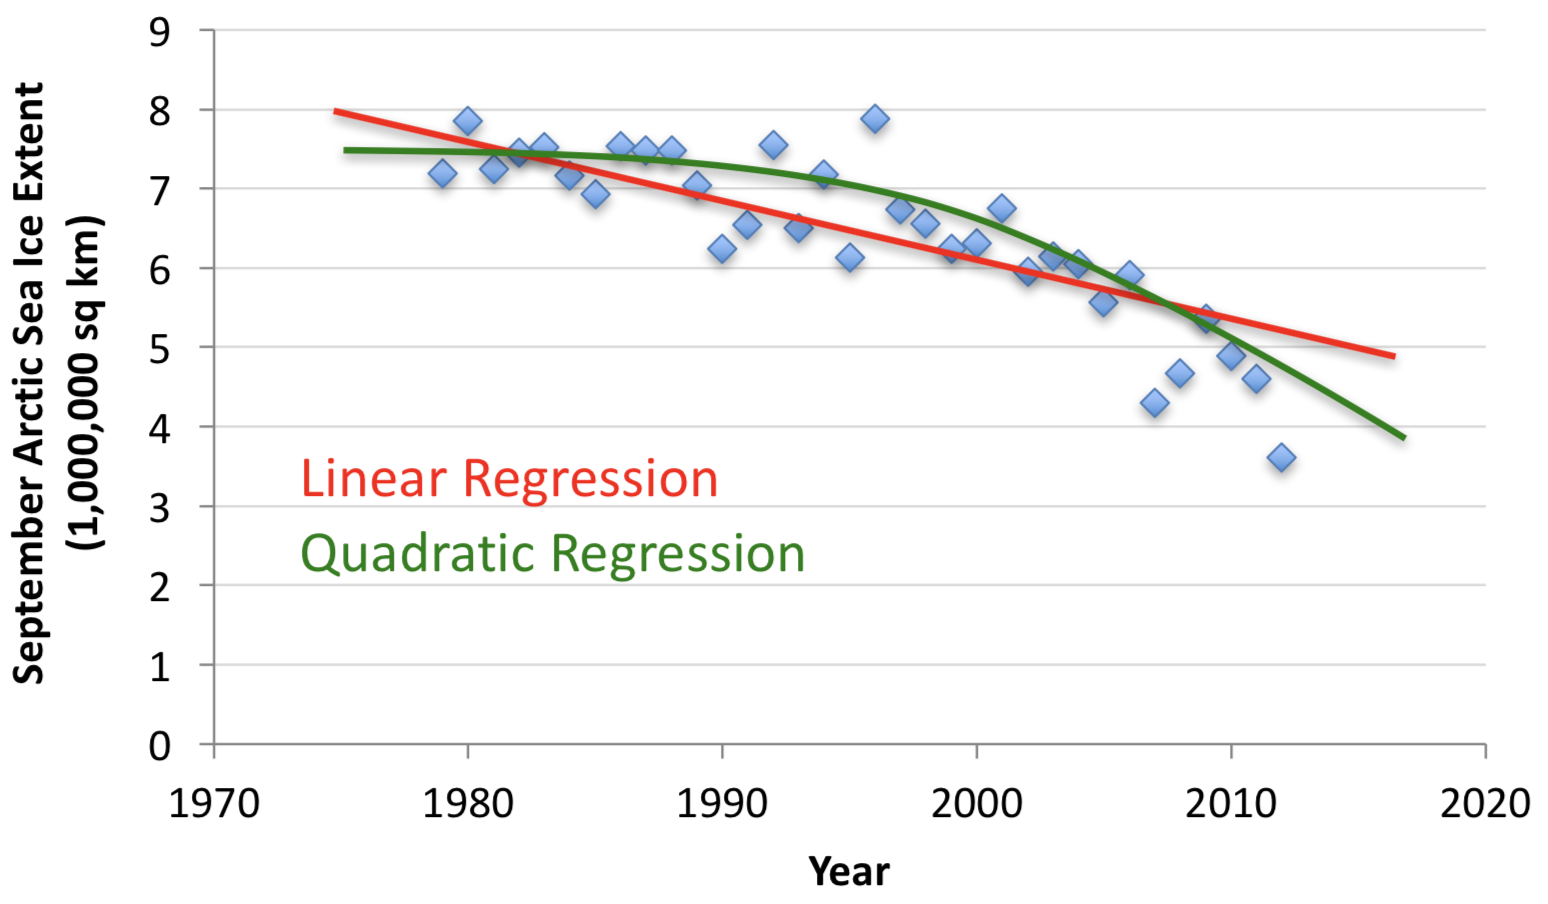
\includegraphics[alt={../../deep learning/slides/september sea ice},height=1.6in]{../../deep-learning/slides/september-sea-ice.png}

\begin{itemize}
\item In linear regression we assume that there is a line that fits the data acceptably well.
\begin{itemize}
\item Simple regression: one input variable, e.g.,  \(f(x; \vec{\theta}) = wx + b\), where \(\vec{\theta} = (w, b)\)
\item Multiple regression: multiple input variables
\item Multivariate regression: multiple output variables
\end{itemize}
\end{itemize}

{[}\textsuperscript{byron}-boots]: \url{https://www.cc.gatech.edu/\~bboots3/CS4641-Fall2018/Lecture3/03\_LinearRegression.pdf}
\section{Example: Credit Scoring}
\label{sec:org3859f0d}

Let's create a credit score based on two variables: age and income (in thousands), which we'll say are real numbers.

\begin{itemize}
\item An input \(\vec{x}\) is a vector in \(\mathbb{R}^2\).  For example, a 25 year-old person making \$60,000 would be represented by the vector \((24, 60)\).

\item "Credit score" = \(\sum_{i=1}^{d} w_i x_i\)
\end{itemize}

The weights \(w_i\) represent the importance of corresponding features of input instances.

From that "score" we take a decision:

\begin{itemize}
\item Approve credit if \(\sum_{i=1}^{d} w_i x_i \ge\) threshold
\item Deny credit if \(\sum_{i=1}^{d} w_i x_i\) < threshold
\end{itemize}
\section{Data Sets}
\label{sec:org077b530}

Consider a hypothetical data set, \(\mathcal{D}\), for the credit scoring problem.

\begin{itemize}
\item Each data point represents a previous customer
\item Since this is is supervised learning, every data point has an associated label: \(+1\) for a customer off whom the bank made money, \(-1\) for a customer off whom the bank lost money
\end{itemize}

\begin{lstlisting}[language=Python,numbers=none]
    age  income  approve
0    64      90        1
1    78      92        1
2    38      80        1
3    29      66       -1
4    94      79        1
\end{lstlisting}

Data in this form is often called a \textbf{design matrix}, an \(N \times D\) matrix in which

\begin{itemize}
\item each of the \(N\) rows represent an example, and
\item each of the \(D\) columns represents a \textbf{feature} (or \textbf{covariate} or \textbf{predictor}) of the data examples.
\end{itemize}
\section{Tabular Data vs. Unstructured Data}
\label{sec:org1b5548e}




The credit data is an example of \textbf{tabular} or \textbf{structured} data.

\begin{lstlisting}[language=Python,numbers=none]
    age  income  approve
0    64      90        1
1    78      92        1
2    38      80        1
3    29      66       -1
4    94      79        1
\end{lstlisting}


We say it is structured because we impose the structure on it.  There is nothing inherent in the data that requires \texttt{age} to come before\textasciitilde{}income\textasciitilde{}, but we must choose some order and stick with it.




\includegraphics[alt={../../deep learning/slides/elsa anna bench.},height=1.8in]{../../deep-learning/slides/elsa-anna-bench.jpeg}


Unstructured data is data whose structure is inherent in the data, not imposed by us.  Examples include images and natural langauge text.
\section{Credit Data Plot}
\label{sec:org4b70193}

A scatter plot gives us intuition about the structure of the data.

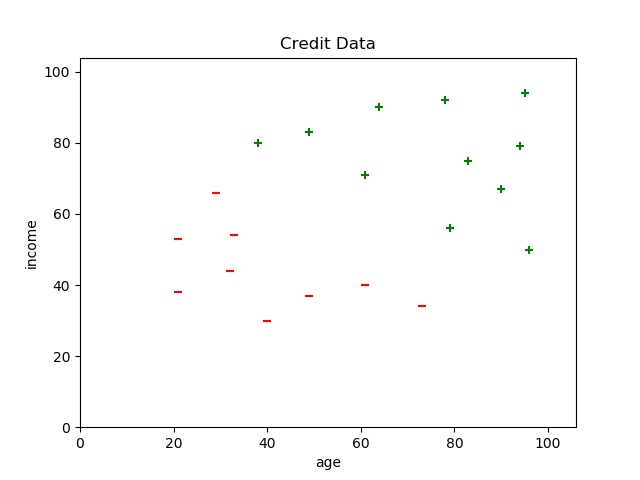
\includegraphics[alt={../../deep learning/slides/credit scatter},height=2.8in]{../../deep-learning/slides/credit-scatter.png}

Is there a line that separates the +s from the -s?
\section{A Linear Separator}
\label{sec:org5ffb106}

Here's a line that separates the data into classes.

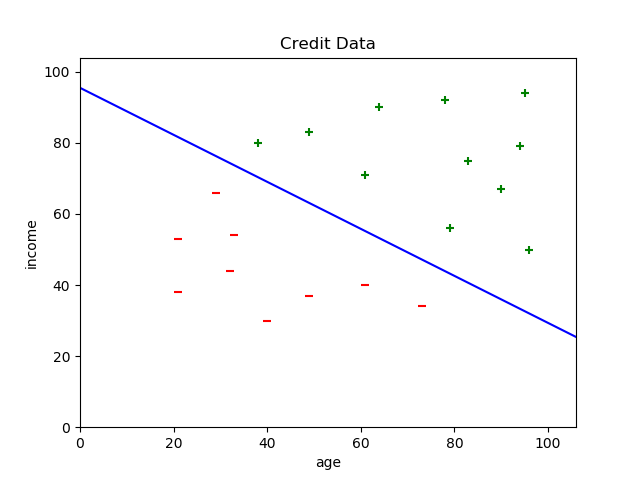
\includegraphics[alt={../../deep learning/slides/credit scatter separator},height=2.8in]{../../deep-learning/slides/credit-scatter-separator.png}

Are there other lines? How many of these lines are there?
\section{Version Spaces}
\label{sec:org1bb0c08}

A \textbf{version space} is the set of all \(h\) in \(\mathcal{H}\) consistent with our training data.  For our credit data, it's the set of all lines that separate the classes.

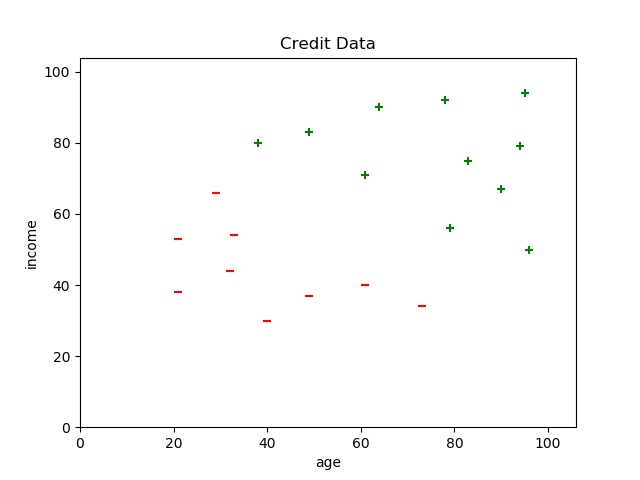
\includegraphics[alt={../../deep learning/slides/credit scatter},height=2.8in]{../../deep-learning/slides/credit-scatter.png}

Machine learning algorithms find these lines algorithmically.
\section{A Practical Example: Iris Classification}
\label{sec:orge011142}

It's a rite of passage to apply supervised learning to the Iris data set. The canonical source for the Iris data set is the \href{https://archive.ics.uci.edu/ml/}{UCI Machine Learning Repository}. Download  \href{https://archive.ics.uci.edu/ml/machine-learning-databases/iris/iris.data}{iris.data}.

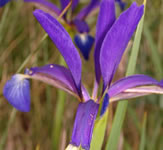
\includegraphics[alt={../../deep learning/slides/iris},height=2.4in]{../../deep-learning/slides/iris.jpg}
\section{Iris Data}
\label{sec:orga613022}

The data set contains 150 instance of Iris flowers with

\begin{itemize}
\item 4 features:
\begin{itemize}
\item sepal\textsubscript{length}
\item sepal\textsubscript{width}
\item petal\textsubscript{length}
\item petal\textsubscript{width}
\end{itemize}
\end{itemize}

and

\begin{itemize}
\item 3 classes:
\begin{itemize}
\item Iris-setosa
\item Iris-versicolour
\item Iris-virginica
\end{itemize}
\end{itemize}
\section{Scikit-learn Recipe}
\label{sec:orga0e01bc}

\begin{enumerate}
\item Set up feature matrix and target array
\item Separate data into training set and test set
\item Choose (import) model class
\item Set model parameters via arguments to model constructor
\item Fit model to data
\item Apply model to new data
\end{enumerate}

Let's apply this recipe to a data set.
\section{Scikit-learn Data Representation}
\label{sec:org59ddf42}

The basic supervised learning setup in Scikit-learn is:

\begin{itemize}
\item Feature Matrix

\begin{itemize}
\item Rows are instances
\item Columns are features
\end{itemize}

\item Target array

\begin{itemize}
\item An array of len(rows) containing the training labels for each instance
\end{itemize}
\end{itemize}

We can easily obtain these with a Pandas DataFrame.
\section{Step 1: Iris feature matix and target array}
\label{sec:orgdbf882e}

From the description on the \href{https://archive.ics.uci.edu/ml/datasets/Iris}{Iris Data Set page} we know that the Iris instances have four features -- (sepal\textsubscript{length}, sepal\textsubscript{width}, petal\textsubscript{length}, petal\textsubscript{width}) -- and three classes -- (Iris-setosa, Iris-versicolour, Iris-virginica). We can read these into a DataFrame with [\textsuperscript{DataLoaders}]

\begin{lstlisting}[language=Python,numbers=none]
import pandas as pd
iris = pd.read_csv(
    "iris.data",
    names=["sepal_length", "sepal_width", "petal_length", "petal_width", "species"])
iris.head()
   sepal_length  sepal_width  petal_length  petal_width      species
0           5.1          3.5           1.4          0.2  Iris-setosa
1           4.9          3.0           1.4          0.2  Iris-setosa
2           4.7          3.2           1.3          0.2  Iris-setosa
3           4.6          3.1           1.5          0.2  Iris-setosa
4           5.0          3.6           1.4          0.2  Iris-setosa
\end{lstlisting}

This DataFrame (in \href{http://vita.had.co.nz/papers/tidy-data.pdf}{tidy format}) contains an \(N \times D\) design matrix in the first four columns.


\href{https://github.com/uci-ml-repo/ucimlrepo}{\^{}DataLoaders]: You can get this data set through Scikit-learn's datasets module or the [ucimlrepo} package, but I want to show the use of Pandas for general data manipulation.
\section{Step 1.1: Scikit-learn Input Data}
\label{sec:orga9749bb}

For Scikit-learn we need a feature matrix \texttt{X} and target array \texttt{y}:

\begin{lstlisting}[language=Python,numbers=none]
X_iris = iris.drop("species", axis=1)
y_iris = iris["species"]
\end{lstlisting}

We can check that the number of samples in the feature matrix equals the number of labels in the target array with

\begin{lstlisting}[language=Python,numbers=none]
X_iris.shape[0] == y_iris.shape[0] # True
\end{lstlisting}

There are 150 samples and 150 target labels.
\section{Step 2: Separate Data into Training and Test Sets}
\label{sec:org8672eb8}

We want to separate our data into non-overlapping training and test subsets. Since the data in our data set are arranged in a neat order, we should randomize the samples and split in a way that represents each class equally in the training and test sets. Scikit-learn provides a library functoin to do this:

\begin{lstlisting}[language=Python,numbers=none]
import sklearn
from sklearn.model_selection import train_test_split

X_iris_train, X_iris_test, y_iris_train, y_iris_test = \
    train_test_split(X_iris,
                     y_iris,
                     random_state=1)
\end{lstlisting}

You will often want to create a third set, a \textbf{validation} set, which you use to tune hyperparameters.

\begin{quote}
Set aside your test set at the beginning of the process and don't use it for anything but testing!
\end{quote}
\section{Step 3.1: Choose a model}
\label{sec:org4700624}

In your machine learning class you'll learn that no hypothesis class (aka model class, aka hypothesis class, aka algorithm, aka estimator) is best for all data [\textsuperscript{fn2}]. You must choose your model class based on the data. Things to consider:

\begin{itemize}
\item What's the dimensinalty of your data?
\item Are your features linearly separable?
\item Are your features numeric or categorical?
\end{itemize}

Scikit-learn calls models \textbf{estimators}.

\href{https://www.cc.gatech.edu/\~isbell/reading/papers/nfl-optimization.pdf}{\^{}fn2]: [Wolpert and Macready, \textbf{No Free Lunch Theorems for Optimization}}
\section{Step 3: Visualizing the Iris data}
\label{sec:org888497f}

You can begin to explore your data with a pairplot:

\begin{lstlisting}[language=Python,numbers=none]
import seaborn as sns
sns.pairplot(X_iris_train, hue="species", size=1.5)
\end{lstlisting}

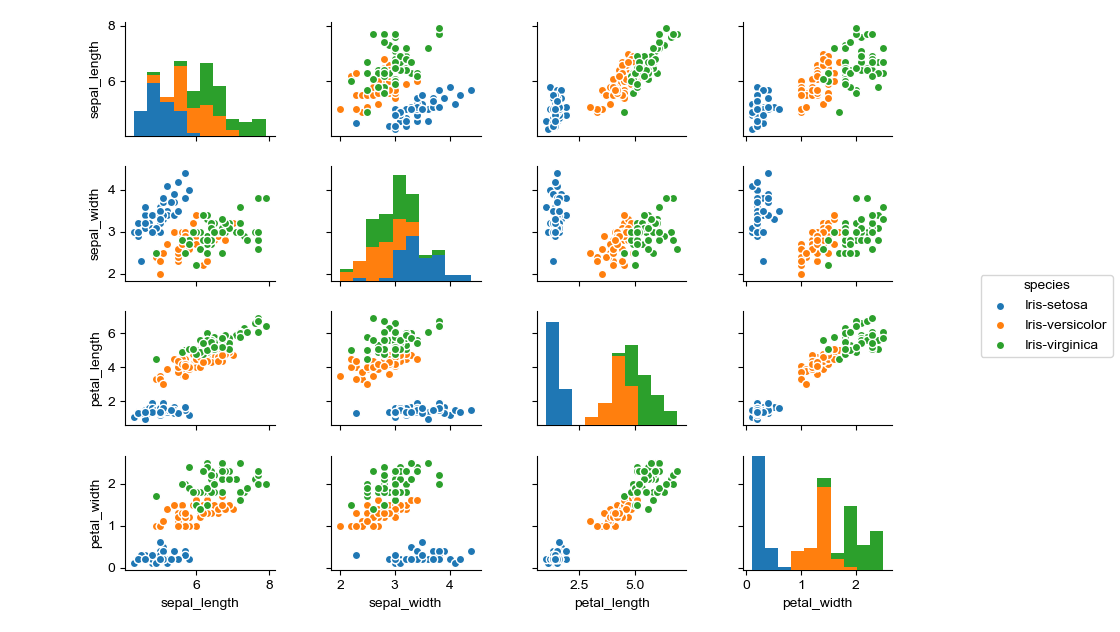
\includegraphics[alt={../../deep learning/slides/iris pairplot},height=2.4in]{../../deep-learning/slides/iris-pairplot.png}

These look linearly separable, so we'll try a linear discriminant classifier, SVM.
\section{Step 4: Set algorithm hyperparameters}
\label{sec:orgcf60879}

Hyperparameters are parameters of the algorithm or fixed parameters of the model, as opposed to the learnable parameters of the model that are adjusted by the learning algorithm.

\begin{lstlisting}[language=Python,numbers=none]
from sklearn import svm
model = svm.SVC(kernel="linear")
\end{lstlisting}

Most parameters are optional, with reasonable default values. Beacuse we know the Iris data set is so well-suited to liner classifiers we choose a \texttt{linear} kernel (deafult is \texttt{rbf} -- radial basis function)
\section{Step 5: Fit model to data}
\label{sec:org94049d3}

The General Form of Learning Algorithms is:

\begin{enumerate}
\item Initialize a model's parameters to some initial values.
\item Until some stopping criterion is reached (e.g., error within bounds)

\begin{itemize}
\item Evaluate the model on some subset of the data \(\mathcal{D}\)
\item If error is present, update the model's parameters to reduce the error
\begin{itemize}
\item The magnitude of the correction is often captured in a "learning rate" hyperparameter, often represented by \(\eta\) or \(\alpha\)
\end{itemize}
\end{itemize}
\end{enumerate}

When the algorithm is finished, you have a model, a particular \(h \in \mathcal{H}\), that "fits" the training data.  In Scikit-learn the learning algorithm is encapsulated in the model's \texttt{fit} method:

\begin{lstlisting}[language=Python,numbers=none]
model.fit(X_iris_train, y_iris_train)
\end{lstlisting}
\section{Step 6: Apply model to new data}
\label{sec:org185a6e5}

To apply the trained model to new (unseen) data, pass an array of instances to \texttt{predict}:

\begin{lstlisting}[language=Python,numbers=none]
y_iris_model = model.predict(X_iris_test)
\end{lstlisting}

We can test the generalization error (how well the classifier performs on unseen data) using the built-in accuracy score:

\begin{lstlisting}[language=Python,numbers=none]
from sklearn.metrics import accuracy_score
accuracy_score(y_iris_test, y_iris_model)
1.0
\end{lstlisting}

As you can see, a linear SVM classifier works perfectly on the Iris data. Try out different classifiers to see how well they perform.

A Scikit-learn estimator (model/hypothesis) is an object that has \texttt{fit} (train) and \texttt{predict} (test) methods.
\section{The Deep Learning Revolution}
\label{sec:org609292f}

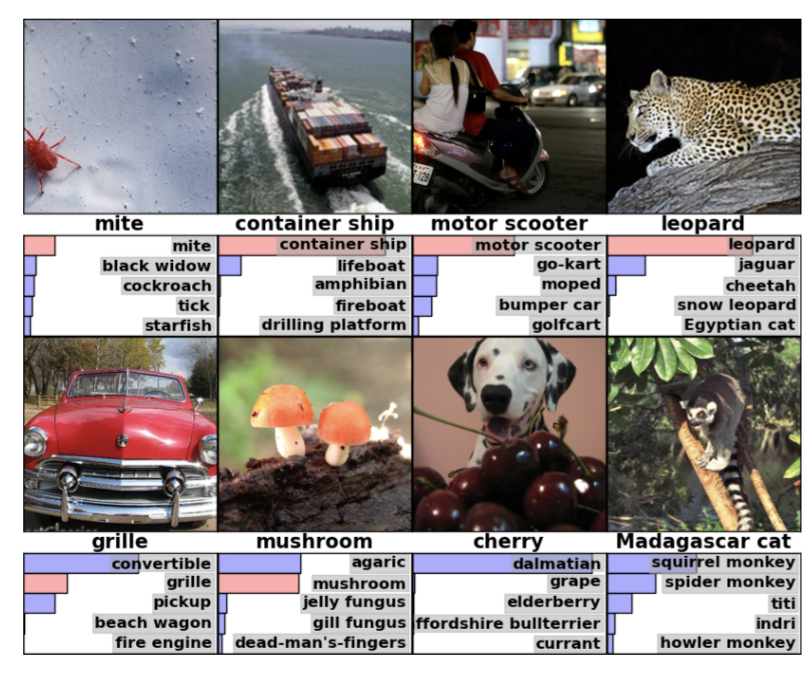
\includegraphics[alt={../../deep learning/slides/imagenet},height=2.4in]{../../deep-learning/slides/imagenet.png}


In 2010, \href{https://profiles.stanford.edu/fei-fei-li}{Fei-Fei Li} and her team published a data set of tens of millions of labeled photographs -- \href{https://image-net.org}{ImageNet} -- and launched the annual ImageNet Large Scale Visual Recognition Challenge (ILSVRC)

In the first two years traditional approaches, characterized by complex feature engineering, continued to win.
\section{AlexNet}
\label{sec:org261e179}

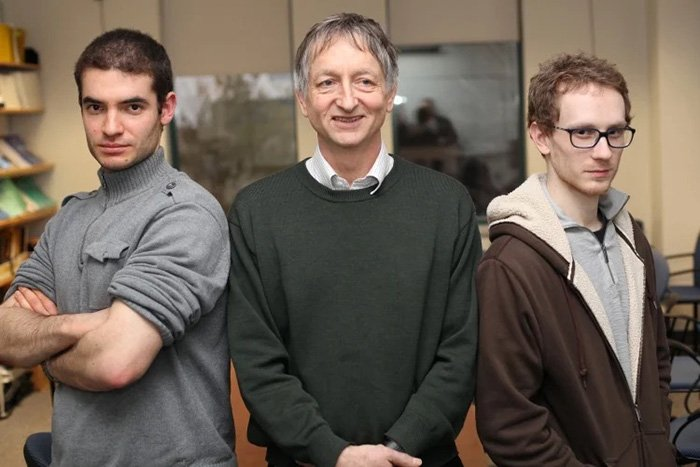
\includegraphics[alt={Ilya Sutskever, Geoff Hinton, Alex Krizhevsky},height=2.0in]{../../deep-learning/slides/ilya-geoff-alex.jpg}

In 2012, Alex Krizhevsky and Ilya Sutskever from Geoff Hinton's lab at the University of Toronto \textbf{dominated} the ILSVRC with what is now called \href{https://www.cs.toronto.edu/\~kriz/imagenet\_classification\_with\_deep\_convolutional.pdf}{AlexNet}

Since then, deep learning has practically taken over AI.


{[}\textsuperscript{UTorontoHintonNobel}]: \url{https://web.cs.toronto.edu/news-events/news/congratulations-pour-in-for-geoffrey-hinton-after-nobel-win}
\section{Autonomous Cars}
\label{sec:org7fec871}

Autonomous cars are teeming with deep learning models.

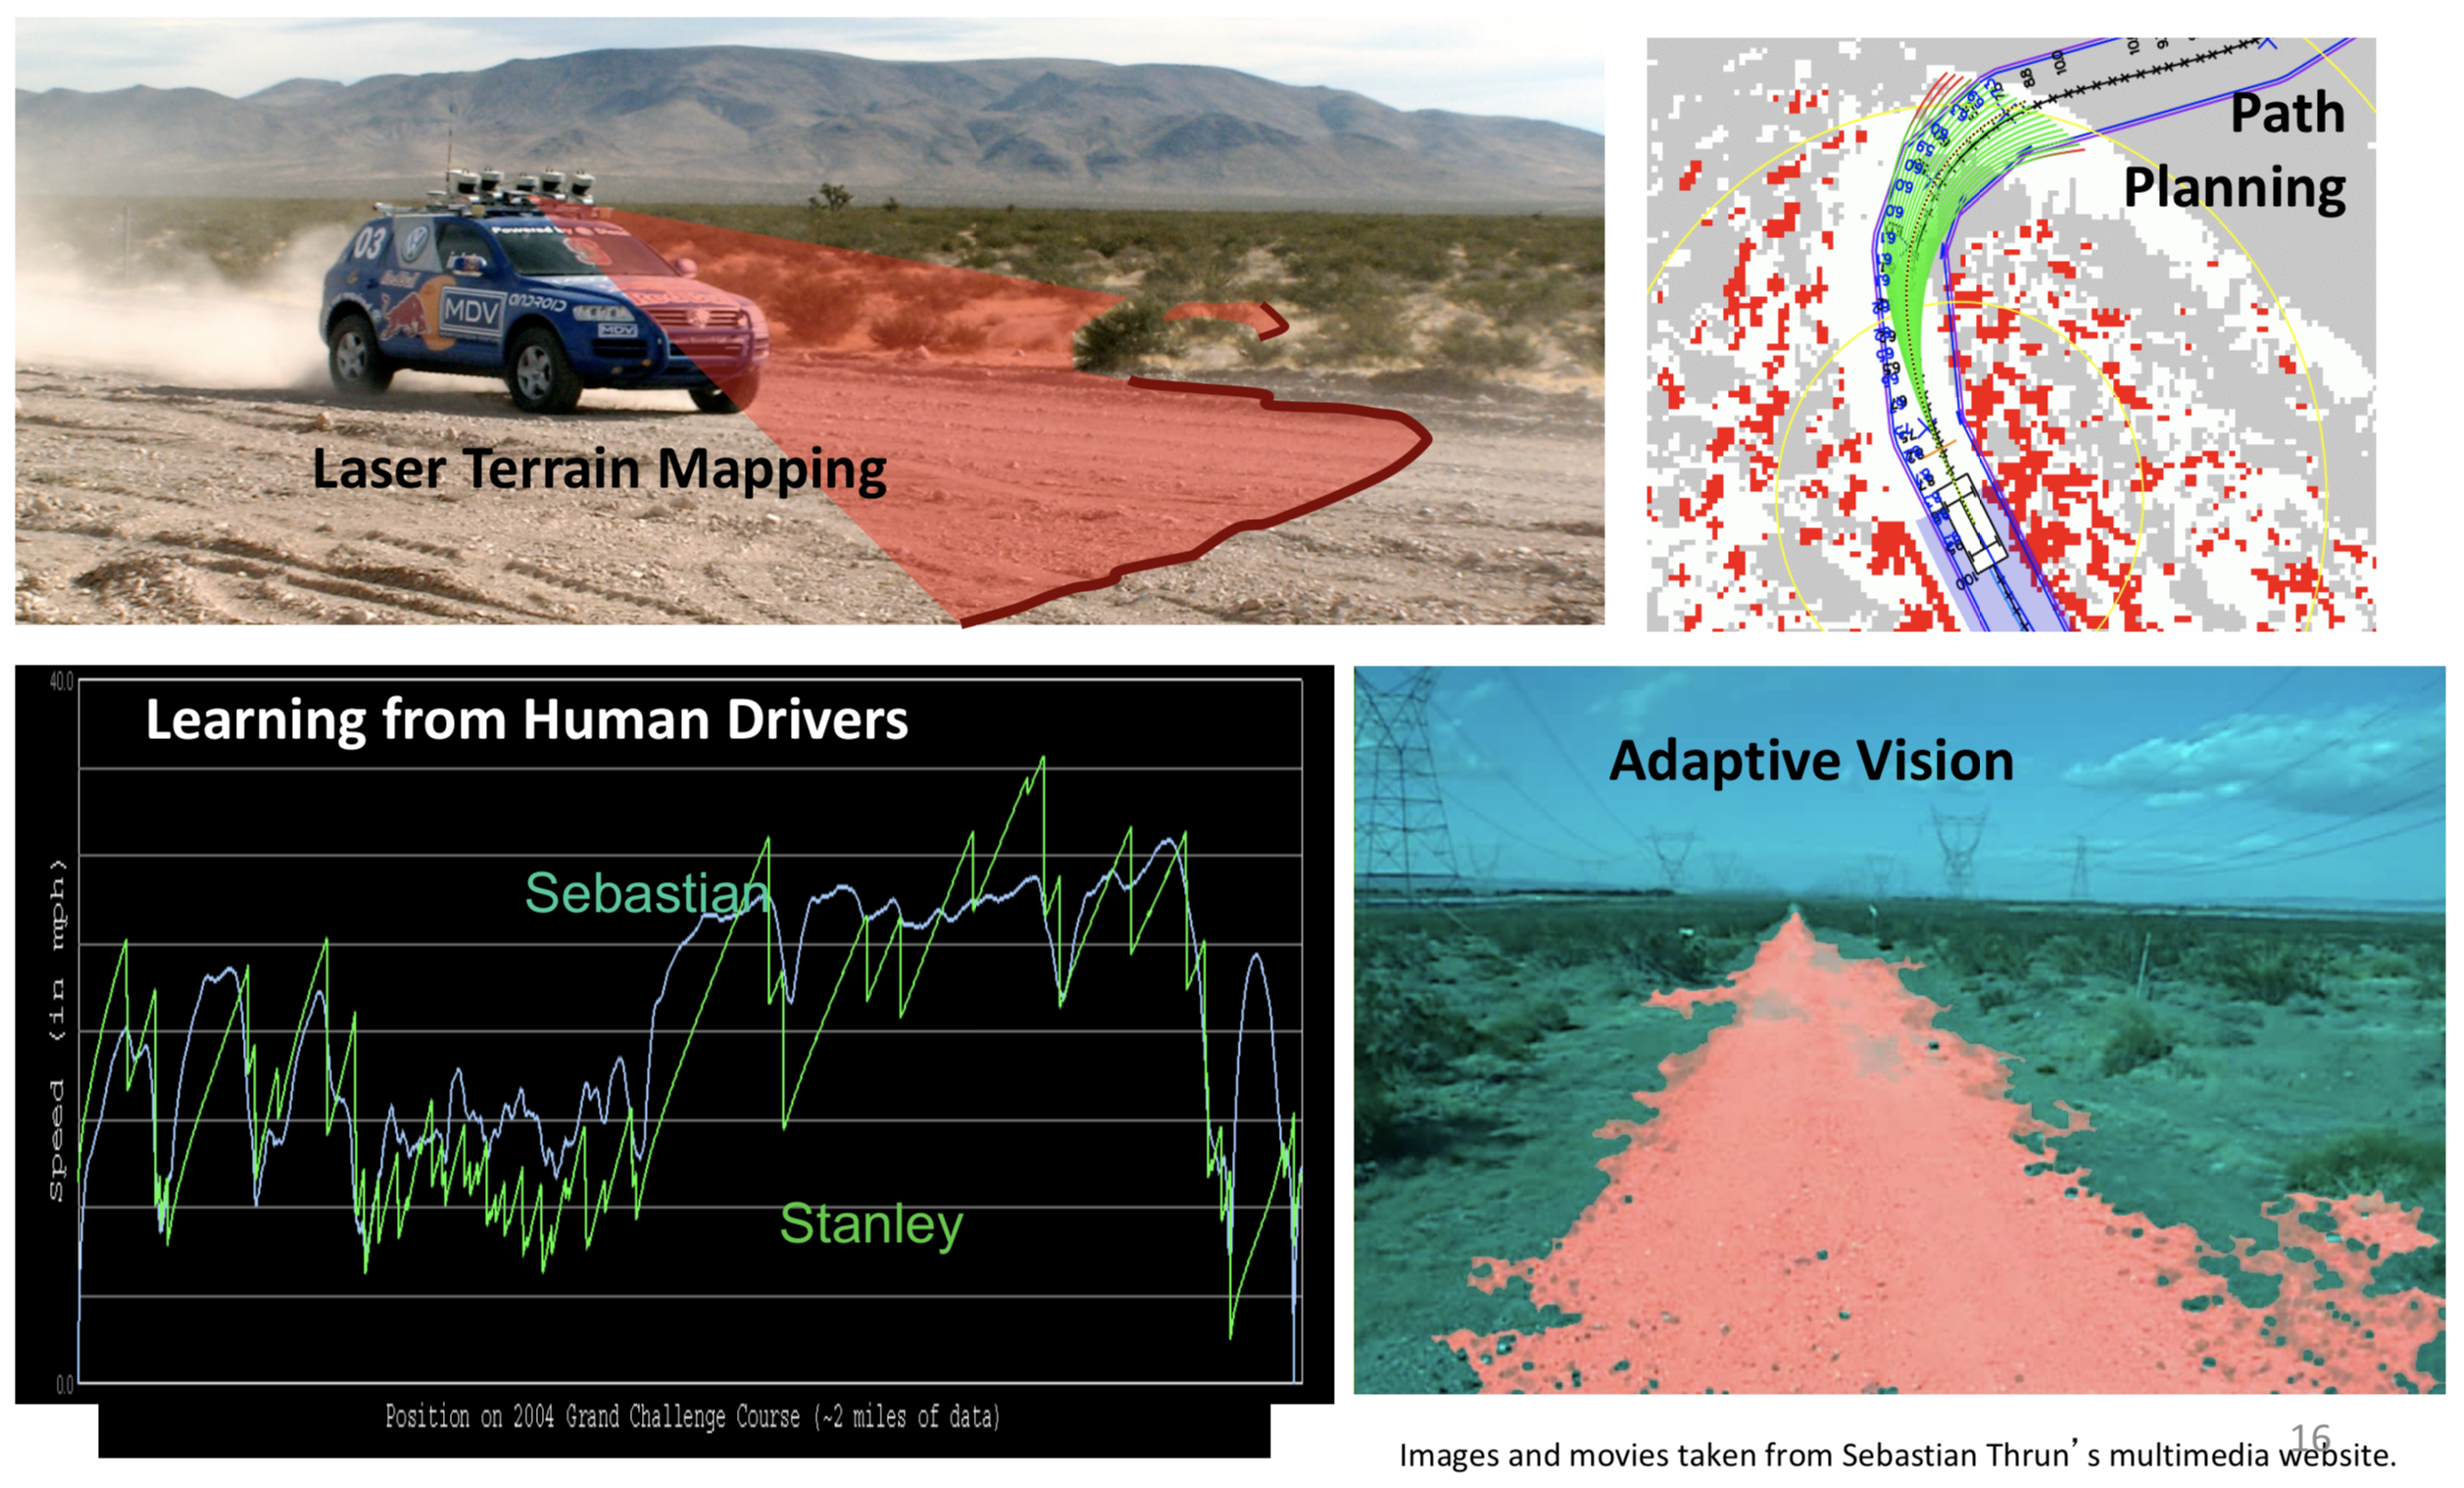
\includegraphics[alt={../../deep learning/slides/thrun autonomous cars},height=3.0in]{../../deep-learning/slides/thrun-autonomous-cars.png}
\section{Scene Labeling}
\label{sec:org24a96c6}

Convolutional deep neural networks (CNNs), or ConvNets, are widely used in vision applications.

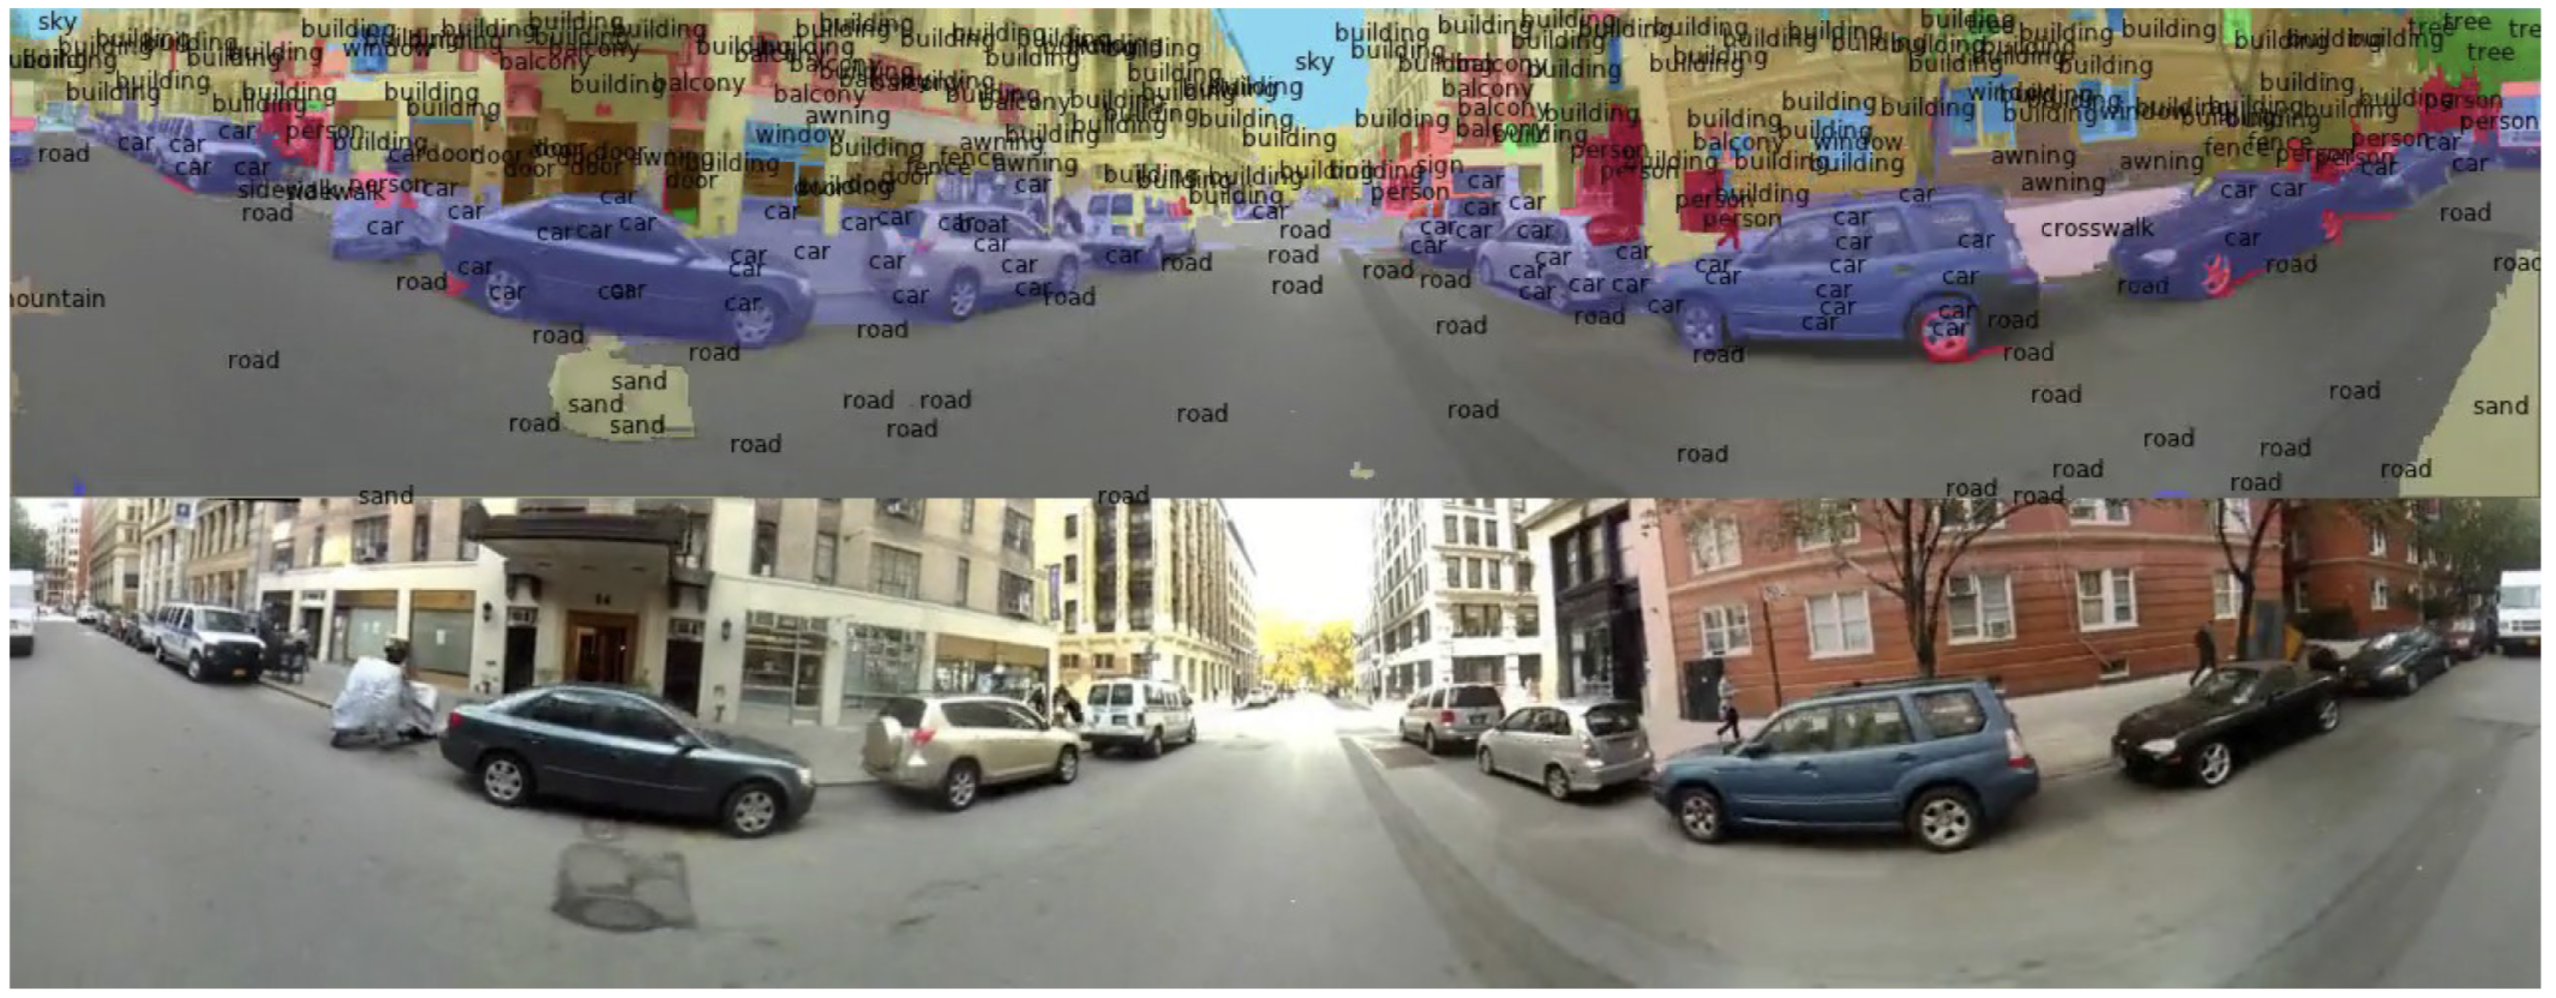
\includegraphics[alt={../../deep learning/slides/farabet scene labeling},height=3.0in]{../../deep-learning/slides/farabet-scene-labeling.png}

{[}\textsuperscript{farabet}]: Farabet et al. ICML 2012, PAMI 2013
\section{Speech Recognition}
\label{sec:org76ff0ce}

One of the early projects that popularized the uses of ReLU activation functions in deep neural networks.

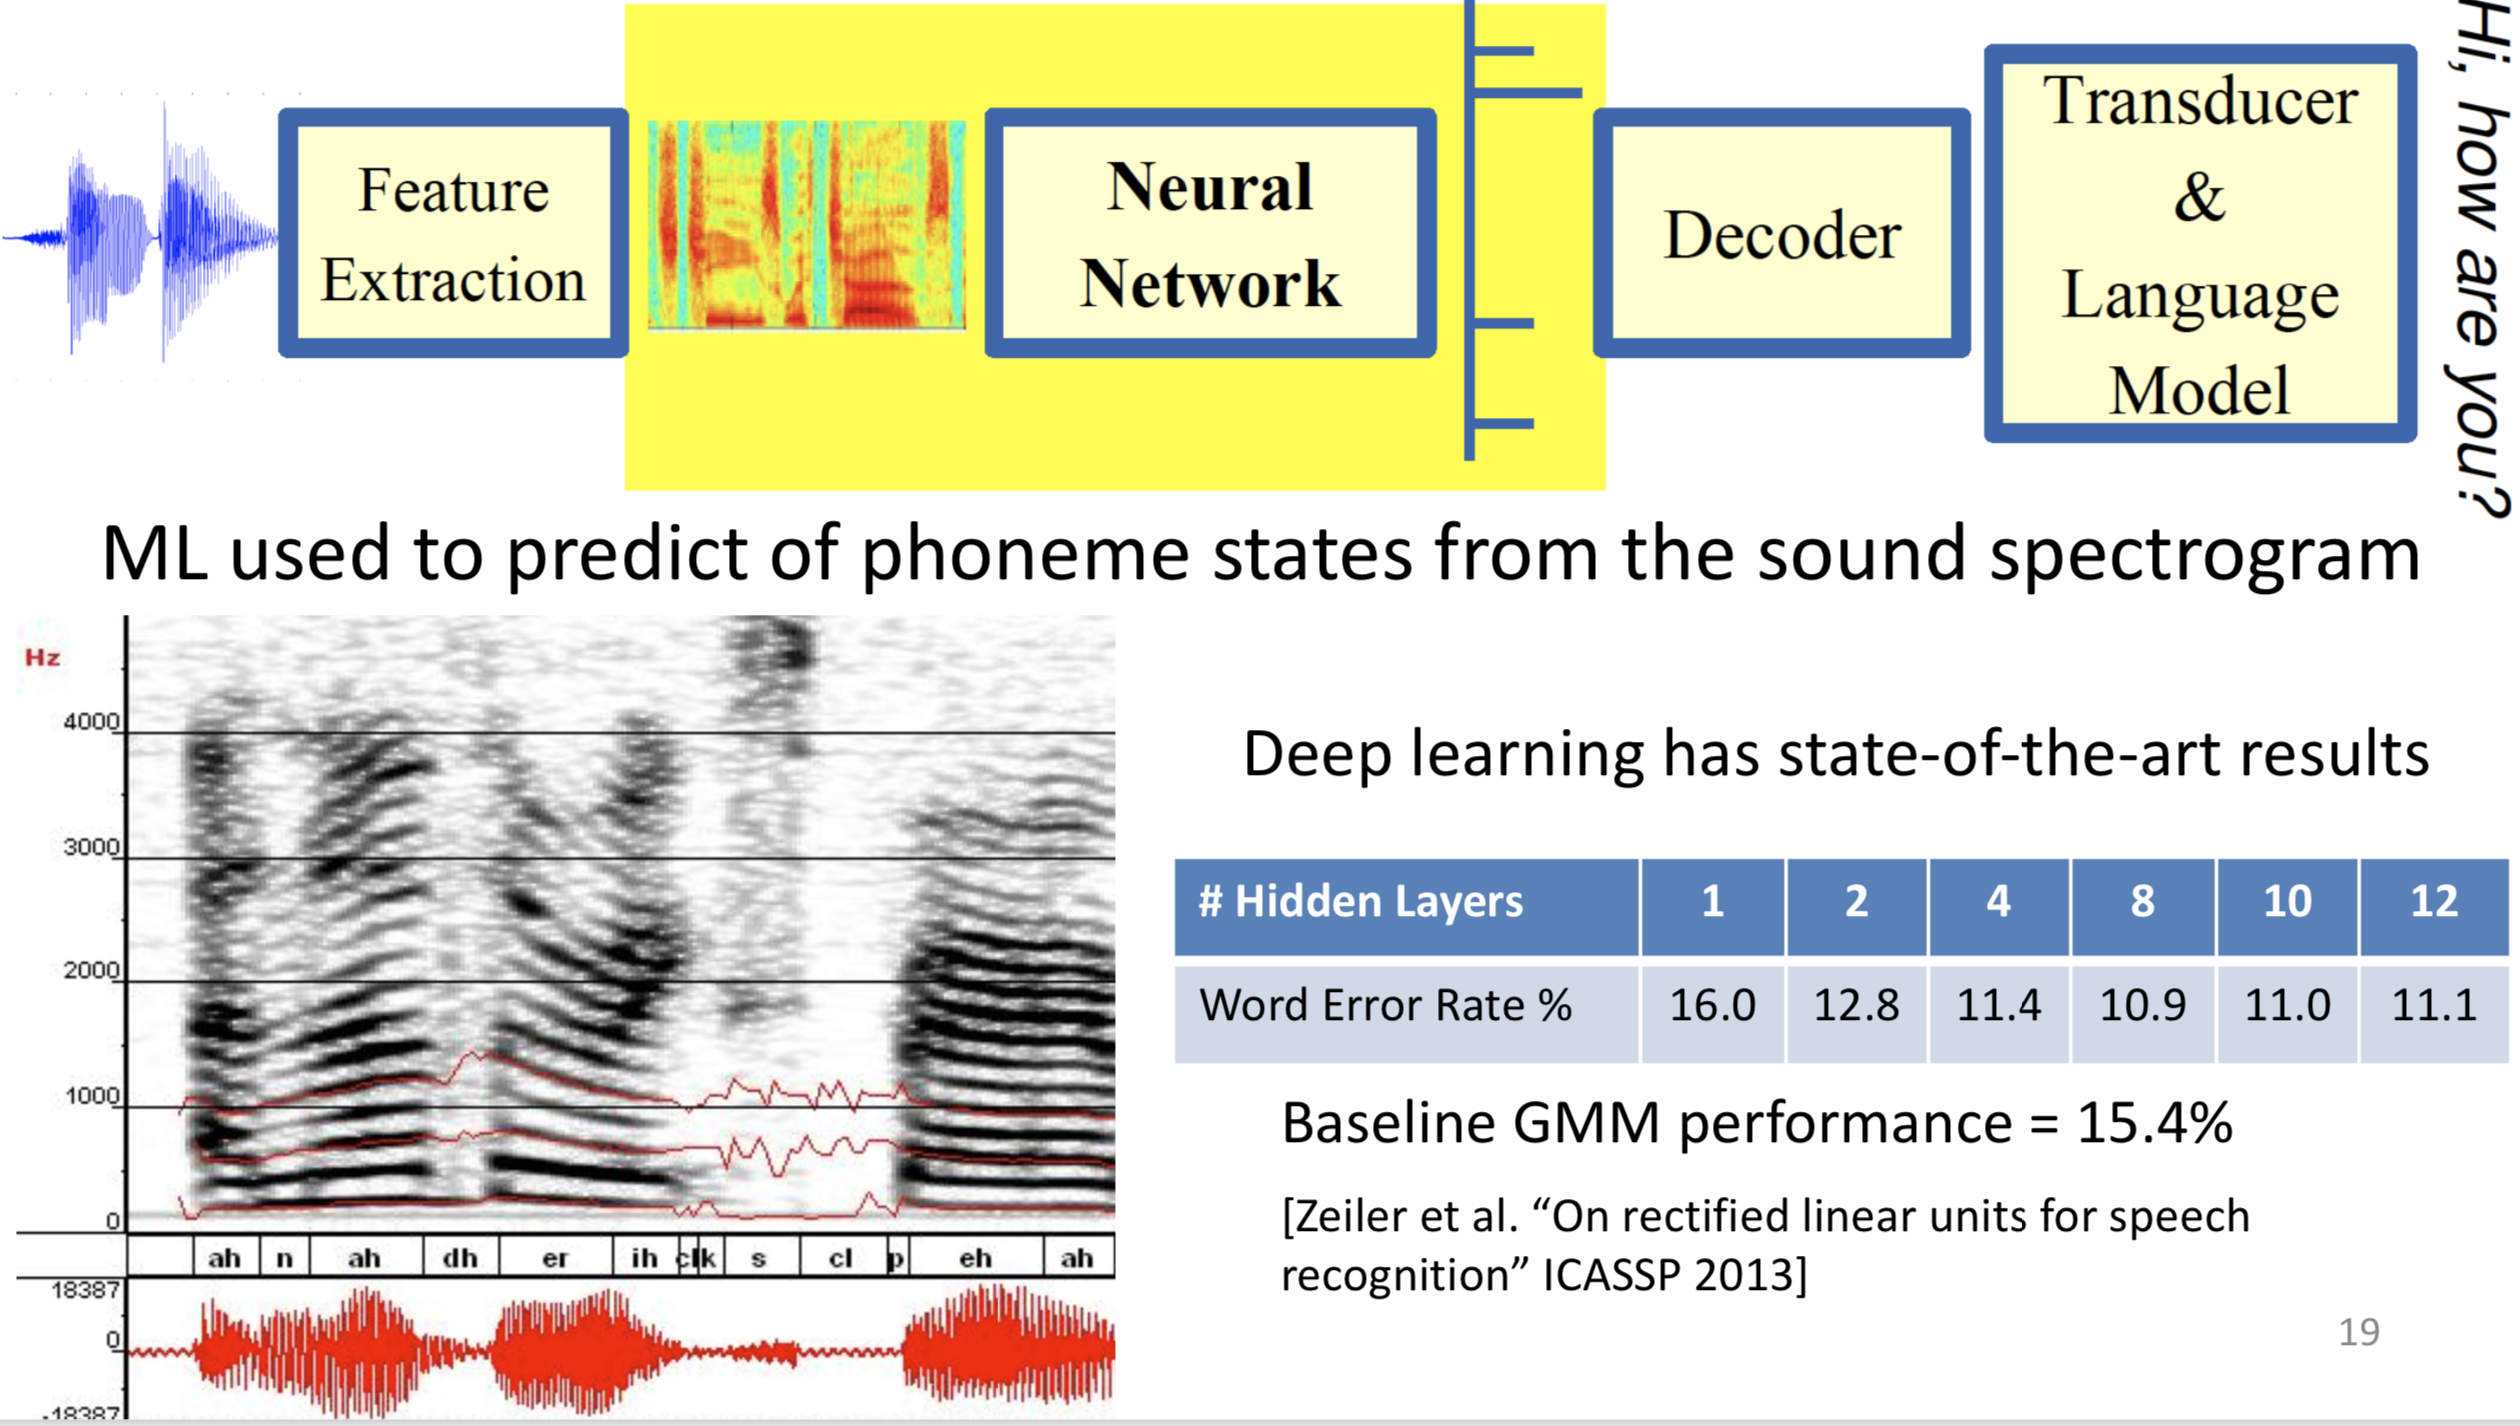
\includegraphics[alt={../../deep learning/slides/zeiler speech recognition},height=3.2in]{../../deep-learning/slides/zeiler-speech-recognition.png}
\section{Generative AI}
\label{sec:org8197f3f}

What is "generative AI?"

\begin{itemize}
\item Two types of supervised machine learning models: discriminative and generative
\begin{itemize}
\item Discriminative, \(p(y|x)\): learn a function that discriminates between classes
\item Generative, \(p(x, y)\): learn a joint probability distribution over data
\begin{itemize}
\item Enables generative models to both discriminate and \textbf{generate samples}
\end{itemize}
\end{itemize}
\item Modern GenAI based on deep learning
\item Gained attention with Ian Goodfellow's generative adversarial networks (GANs) in 2014, now auto-regressive transformer models all the rage, e.g., large language models (LLMs) like ChatGPT
\end{itemize}
\end{document}
